% ------------------------------------------------------------------------------
% TYPO3 CMS 6.2 LTS - What's New - Chapter "Responsive Images" (German Version)
%
% @author	Michael Schams <schams.net>
% @license	Creative Commons BY-NC-SA 3.0
% @link		http://typo3.org/download/release-notes/whats-new/
% @language	German
% ------------------------------------------------------------------------------
% Chapter: Responsive Images
% ------------------------------------------------------------------------------

\section{Responsive Images}
\begin{frame}[fragile]
	\frametitle{Responsive Images}

	\begin{center}\huge{Kapitel 2:}\end{center}
	\begin{center}\huge{\color{typo3darkgrey}\textbf{Responsive Images}}\end{center}

\end{frame}

% ------------------------------------------------------------------------------
% Select Screen Size In Page Preview
% ------------------------------------------------------------------------------

\begin{frame}[fragile]
	\frametitle{Responsive Images}
	\framesubtitle{Bildschirmgrößen in der Seitenvorschau}

	\begin{itemize}
		\item Redakteure können nun verschiedene Bildschirmgrößen (Breiten) für die Vorschau auswählen, um responsive Websites testen zu können
	\end{itemize}

	\begin{figure}
		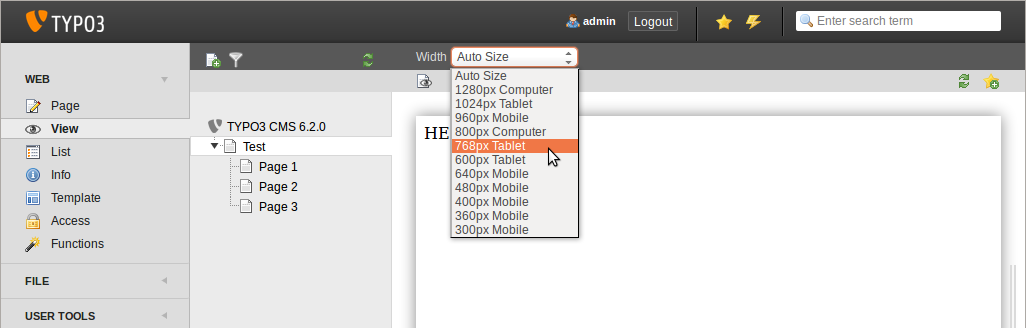
\includegraphics[width=0.95\linewidth]{Images/ResponsiveImages/ScreenSizeInPagePreview.png}
	\end{figure}

\end{frame}

% ------------------------------------------------------------------------------
% Customize Available Screen Sizes
% ------------------------------------------------------------------------------

\begin{frame}[fragile]
	\frametitle{Responsive Images}
	\framesubtitle{Bildschirmgrößen in der Seitenvorschau}

	\begin{itemize}
		\item Bildschirmgrößen sind via PageTSconfig konfigurierbar:

		\lstset{
			basicstyle=\fontsize{7}{9}\selectfont\ttfamily
		}

		\begin{lstlisting}
			mod.web_view.previewFrameWidths {
			  1780.label = <any LLL or string>
			  1780.height = 145
			}
		\end{lstlisting}

		\item Der Schlüssel (hier: 1780) gibt die Breite an, die Höhe (height) ist optional
		\item Vorgegebene Größen sind in der folgenden Datei definiert:\newline
			\small\texttt{typo3/sysext/core/Configuration/DefaultConfiguration.php}\normalsize
		\item Labels können via PageTSconfig konfiguriert werden:

		\begin{lstlisting}
			mod.web_view.previewFrameWidths {
			  1280.label = LLL:EXT:viewpage/Resources/Private/Language/locallang.xlf:computer
			  1024.label = LLL:EXT:viewpage/Resources/Private/Language/locallang.xlf:tablet
			}
		\end{lstlisting}

	\end{itemize}

\end{frame}

% ------------------------------------------------------------------------------
% Responsive Image Galleries
% ------------------------------------------------------------------------------

\begin{frame}[fragile]
	\frametitle{Responsive Images}
	\framesubtitle{Responsive Bildergalerien}

	\begin{itemize}
		\item Es wurden zusätzliche Attribute für responsive Bildergalerien eingeführt
		\item Dafür wurde das Rendering von "CSS styled content" erweitert
		\item Beispiel: HTML5 (\texttt{config.doctype = html5} vorausgesetzt)\newline

			TYPO3 CMS vor 6.2:

			\lstset{
				basicstyle=\fontsize{7}{9}\selectfont\ttfamily
			}

			\begin{lstlisting}
				<div class="csc-textpic-imagewrap">...</div>
			\end{lstlisting}

			TYPO3 CMS ab 6.2:

			\begin{lstlisting}
				<div class="csc-textpic-imagewrap"
				  data-csc-images="{register:imageCount}"
				  data-csc-cols="{field:imagecols}">...</div>
			\end{lstlisting}

	\end{itemize}

\end{frame}

% ------------------------------------------------------------------------------
% Responsive Image Rendering
% ------------------------------------------------------------------------------

\begin{frame}[fragile]
	\frametitle{Responsive Images}
	\framesubtitle{Responsive Image Rendering}

	\begin{itemize}
		\item cObject IMAGE kann nun so genannte "sourceCollections" rendern, um damit verschiedene Display-Auflösungen und Bildschirmgrößen zu unterstützen
		\item Zum Aktivieren des responsive Image Rendering für die cObjects "Bild" und "Text/Bild" müssen folgende Einstellungen gemacht werden:

			\texttt{styles.content.imgtext.responsive}\newline
			\texttt{styles.content.imgtext.layoutKey}

		\item Gültige ("out of the box") Optionen sind:

			\begin{itemize}
				\item \texttt{default}:	\tabto{2cm} standard \texttt{<img>}-tag
				\item \texttt{srcset}:	\tabto{2cm} \texttt{<img>}-tag mit alternativer Bildquelle als srcset-Attribut
				\item \texttt{picture}:	\tabto{2cm} \texttt{<picture>}-tag mit source-child-tags
				\item \texttt{data}:	\tabto{2cm} \texttt{<img>}-tag mit alternativer Bildquelle as data-Attribut
			\end{itemize}

	\end{itemize}

\end{frame}

% ------------------------------------------------------------------------------
% Property: layoutKey
% ------------------------------------------------------------------------------

\begin{frame}[fragile]
	\frametitle{Responsive Images}
	\framesubtitle{Eigenschaft: layoutKey}

	\begin{itemize}
		\item \texttt{layoutKey} definiert das Render-Layout\newline
			\small(HTML Code, der für das \texttt{<img>}-tag verwendet wird)\normalsize
		\item Jede Möglichkeit repräsentiert eine unterschiedliche Lösung um HTML-Code für das IMAGE zu rendern
		\item Option \texttt{default} rendert das \texttt{<img>}-tag auf herkömmliche Weise\newline
			\small(jenes empfiehlt sich, wenn das Frontend nicht "responsive" ist)\normalsize
		\item Wenn man ein responsive Layout implementiert, benötigt man unterschiedliche Bildgrößen
		\item Abhängig vom HTML Framework, dem Browser und der JavaScript Bibliothek für das progressive enhancement, verwendet man:

			\begin{itemize}
				\item entweder eines der vordefinierten Layouts,
				\item oder definiert ein neues Layout mit einem neuen layoutKey
			\end{itemize}

	\end{itemize}

\end{frame}

% ------------------------------------------------------------------------------
% Property: layout
% ------------------------------------------------------------------------------

\begin{frame}[fragile]
	\frametitle{Responsive Images}
	\framesubtitle{Eigenschaft: layoutKey}

	\lstset{
		basicstyle=\tiny\ttfamily
	}

	\begin{lstlisting}
		layoutKey = {$styles.content.imgtext.layoutKey}
		layout {
		  default {
		    element = <img src="###SRC###" width="###WIDTH###" height="###HEIGHT###" ###PARAMS###
		      ###ALTPARAMS### ###BORDER######SELFCLOSINGTAGSLASH###>
		  }
		  srcset {
		    element = <img src="###SRC###" srcset="###SOURCECOLLECTION###" ###PARAMS###
		      ###ALTPARAMS### ###SELFCLOSINGTAGSLASH###>
		    source = |*|###SRC### ###SRCSETCANDIDATE###,|*|###SRC### ###SRCSETCANDIDATE###
		  }
		  picture {
		    element = <picture>###SOURCECOLLECTION###<img src="###SRC###" ###PARAMS###
		      ###ALTPARAMS######SELFCLOSINGTAGSLASH###></picture>
		    source = <source src="###SRC###" media="###MEDIAQUERY###"###SELFCLOSINGTAGSLASH###>
		  }
		  data {
		    element = <img src="###SRC###" ###SOURCECOLLECTION### ###PARAMS###
		      ###ALTPARAMS######SELFCLOSINGTAGSLASH###>
		    source = data-###DATAKEY###="###SRC###"
		  }
		}
	\end{lstlisting}

\end{frame}

% ------------------------------------------------------------------------------
% Property: layout.[layoutKey].element
% ------------------------------------------------------------------------------

\begin{frame}[fragile]
	\frametitle{Responsive Images}
	\framesubtitle{Eigenschaft: layout.[layoutKey].element}

	\begin{itemize}
		\item \lstinline!###SRC###!\newline
			URL für Attribut: \texttt{src}

		\item \lstinline!###WIDTH###!\newline
			Bildbreite (in Pixel) für Attribut: \texttt{width}

		\item \lstinline!###HEIGHT###!\newline
			Bildhöhe (in Pixel) für Attribut: \texttt{height}

		\item \lstinline!###PARAMS###!\newline
			Zusätzliche Parameter, wie im cObject IMAGE definiert

		\item \lstinline!###ALTPARAMS###!\newline
			Zusätzliche alternative Parameter, wie im cObject IMAGE definiert

	\end{itemize}

\end{frame}

% ------------------------------------------------------------------------------
% Property: layout.[layoutKey].element
% ------------------------------------------------------------------------------

\begin{frame}[fragile]
	\frametitle{Responsive Images}
	\framesubtitle{Eigenschaft: layout.[layoutKey].element}

	\begin{itemize}
		\item \lstinline!###BORDER###!\newline
			Rahmenbreite (in Pixel) für Attribut: \texttt{border}

		\item \lstinline!###SELFCLOSINGTAGSLASH###!\newline
			Schließendes Tag, z.B. \texttt{<img ... />} oder \texttt{<img ... >}\newline
			(abhängig von \texttt{config.xhtmlDoctype} oder \texttt{config.doctype})

		\item \lstinline!###SOURCECOLLECTION###!\newline
			Zusätzliche Sourcen des Bildes, abhängig von der unterschiedlichen Verwendung im Responsive Web Design.\newline
			Die Werte werden im Schlüssel \texttt{layout.[layoutKey].source} definiert
	\end{itemize}

\end{frame}

% ------------------------------------------------------------------------------
% Property: sourceCollection.[dataKey]
% ------------------------------------------------------------------------------

\begin{frame}[fragile]
	\frametitle{Responsive Images}
	\framesubtitle{Eigenschaft: sourceCollection.[dataKey]}

	\begin{itemize}
		\item Standard sourceCollection von EXT:css\_styled\_content
		\item Es ist zu empfehlen, eine eigene sourceCollection zu erstellen

			\lstset{
				basicstyle=\tiny\ttfamily
			}

			\begin{lstlisting}
				sourceCollection {
				  small {
				    width = 200
				    srcsetCandidate = 600w
				    mediaQuery = (max-device-width: 600px)
				    dataKey = small
				  }
				  smallRetina {
				    if.directReturn = 1
				    width = 200
				    pixelDensity = 2
				    srcsetCandidate = 600w 2x
				    mediaQuery = (max-device-width: 600px) AND (min-resolution: 192dpi)
				    dataKey = smallRetina
				  }
				}
			\end{lstlisting}
	\end{itemize}

\end{frame}

% ------------------------------------------------------------------------------
% Further Resources (External Links)
% ------------------------------------------------------------------------------

\begin{frame}[fragile]
	\frametitle{Responsive Images}
	\framesubtitle{Weitere Informationen}

	\begin{itemize}
		\item Lauffähiges Code-Beispiel:\newline
			\small\url{http://wiki.typo3.org/Responsive_Image_Rendering}\normalsize

		\item Artikel von Sven Wolfermann auf typo3.org:\newline
			\small\url{http://typo3.org/news/article/responsive-image-rendering-in-typo3-cms-62/}\normalsize

		\item W3C Spezifikation:\newline
			\small\url{http://www.w3.org/html/wg/drafts/srcset/w3c-srcset/}\newline
			\small\url{http://www.w3.org/TR/html-picture-element/}

		\item Arbeitsentwurf (working draft) der "Responsive Image Community Group":\newline
			\small\url{http://responsiveimages.org}\normalsize

	\end{itemize}

\end{frame}

% ------------------------------------------------------------------------------

